% vim: tw=80

\chapter{Measurement of the Triple-Differential Dijet Cross Section}

\section{Datasets}
\label{sec:datasets}

\subsection{Data Samples}

The analysis is based on the 2012 data set collected by CMS at a center-of-mass
energy of $\sqrt{s} = 8 \si{\TeV}$. The data sample corresponds to a total integrated
luminosity of $\mathcal{L} = 19.71 \si{\fbinv}$. The integrated luminosity was calculated using
the pixelLumiCalc tool and the recommended golden JSON file.

The primary datasets as shown in Table~\ref{tab:datasets} are used. While in run A all
events were stored in the stream \emph{Jet}, the prescaled and unprescaled triggers were
split into separate streams \emph{JetMon} and \emph{JetHT} in the runs B, C and D.

\begin{table}[htbp]
    \centering
    \begin{tabular}{llll}
    \hline\hline
    Run Period & Run Range & Dataset & Luminosity (\si{\fbinv})\\\hline
    A & 190456--193621 & /Jet/Run2012A-22Jan2013-v1/AOD & 0.88\\
    B & 193834--196531 & /Jet[Mon,HT]/Run2012B-22Jan2013-v1/AOD & 4.49\\
    C & 198022--203742 & /Jet[Mon,HT]/Run2012C-22Jan2013-v1/AOD & 7.06 \\
    D & 203777--208686 & /Jet[Mon,HT]/Run2012C-22Jan2013-v1/AOD & 7.37\\ 
    \hline\hline
    \end{tabular}
    \caption{The full 2012 dataset is used. In Run A, events of all single jet trigger paths are stored in 
        the stream Jet, while the prescaled triggers were moved to the JetMon stream in the runs
        B, C and D. Events triggering the unprescaled trigger are in the stream JETHT.}
    \label{tab:datasets}
\end{table}

The certified runs and lumisections which ensure a high quality of the data are selected using the official
recommended JSON file:

\begin{verbatim}
Cert_190456-208686_8TeV_22Jan2013ReReco_Collisions12_JSON.txt
\end{verbatim}

To compare the data distributions with simulated events, two Monte-Carlo samples were used.
The Madgraph+P6 sample is a multi-leg improved HT-binned sample with a very high number of events. 
The P8 sample is binned in $\hat \pt$ and is based on the $2 \rightarrow 2$ LO QCD process. Both samples
are fully processed using the whole CMSSW event processing chain including a detector simulation.

\begin{table}[htbp]
    \centering
    \begin{tabular}{llll}
    \hline\hline
    Dataset Name & Dataset identifier & Number of events\\\hline
    MG+P6 & /QCD\_HT-XXToXX\_TuneZ2star\_8TeV-madgraph-pythia/Summer12\_DR53X-PU\_S10\_START53\_V7A-v1/AODSIM & \\
    P8 & QCD\_Pt-XXtoXX\_Tune4C\_8TeV\_pythia8/Summer12\_DR53X-PU\_S10\_START53\_V7A-v1/AODSIM & \\
    \hline\hline
    \end{tabular}
    \caption{Official MC production samples used in the analysis.}
    \label{tab:datasets}
\end{table}


\section{Event selection}

\subsection{Trigger studies}

For measuring the data spectrum, the set of single jet triggers was used. Due to
the steep falling jet-\pt spectrum resulting in very large event rates at the
low-\pt end of the spectrum and only a few events at the high-\pt end, the
spectrum is split into mutually excluding regions in which one, fully efficient,
trigger is used. The set of triggers consists of the following trigger paths,
each accepting events with at least one jet with a transverse momentum  large
than $x \si{\GeV}$.

\begin{table}[htbp]
    \centering
    \begin{tabular}{lcccr}
        \toprule
        Trigger path  & L1 (\si{\GeV}) & HLT (\si{\GeV}) & $p_{\mathrm{T},.99\%}$ (\si{\GeV}) & Eff. Lumi \\\midrule
        HLT\_PFJet40  & 16                  & 40                   & --                     & 0.08 \si{\pbinv}\\
        HLT\_PFJet80  & 36                  & 80                   & 123                    & 2.12 \si{\pbinv}\\
        HLT\_PFJet140 & 68                  & 140                  & 192                    & 55.67 \si{\pbinv}\\
        HLT\_PFJet200 & 92                  & 200                  & 263                    & 0.26 \si{\si{\fbinv}}\\
        HLT\_PFJet260 & 128                 & 260                  & 353                    & 1.06 \si{\si{\fbinv}}\\
        HLT\_PFJet320 & 128                 & 320                  & 412                    & 19.71 \si{\si{\fbinv}}\\
        \bottomrule
    \end{tabular}
    \caption{Used trigger paths in the analysis. Each path is used in an mutually exclusive phase space in \ptavg. The
            $p_{\mathrm{T},.99\%}$ threshold gives the value at which a trigger reaches 99\% efficiency compared to lower
            reference trigger.}

    \label{tab:triggers}
\end{table}


\begin{figure}[htbp]
    \centering
    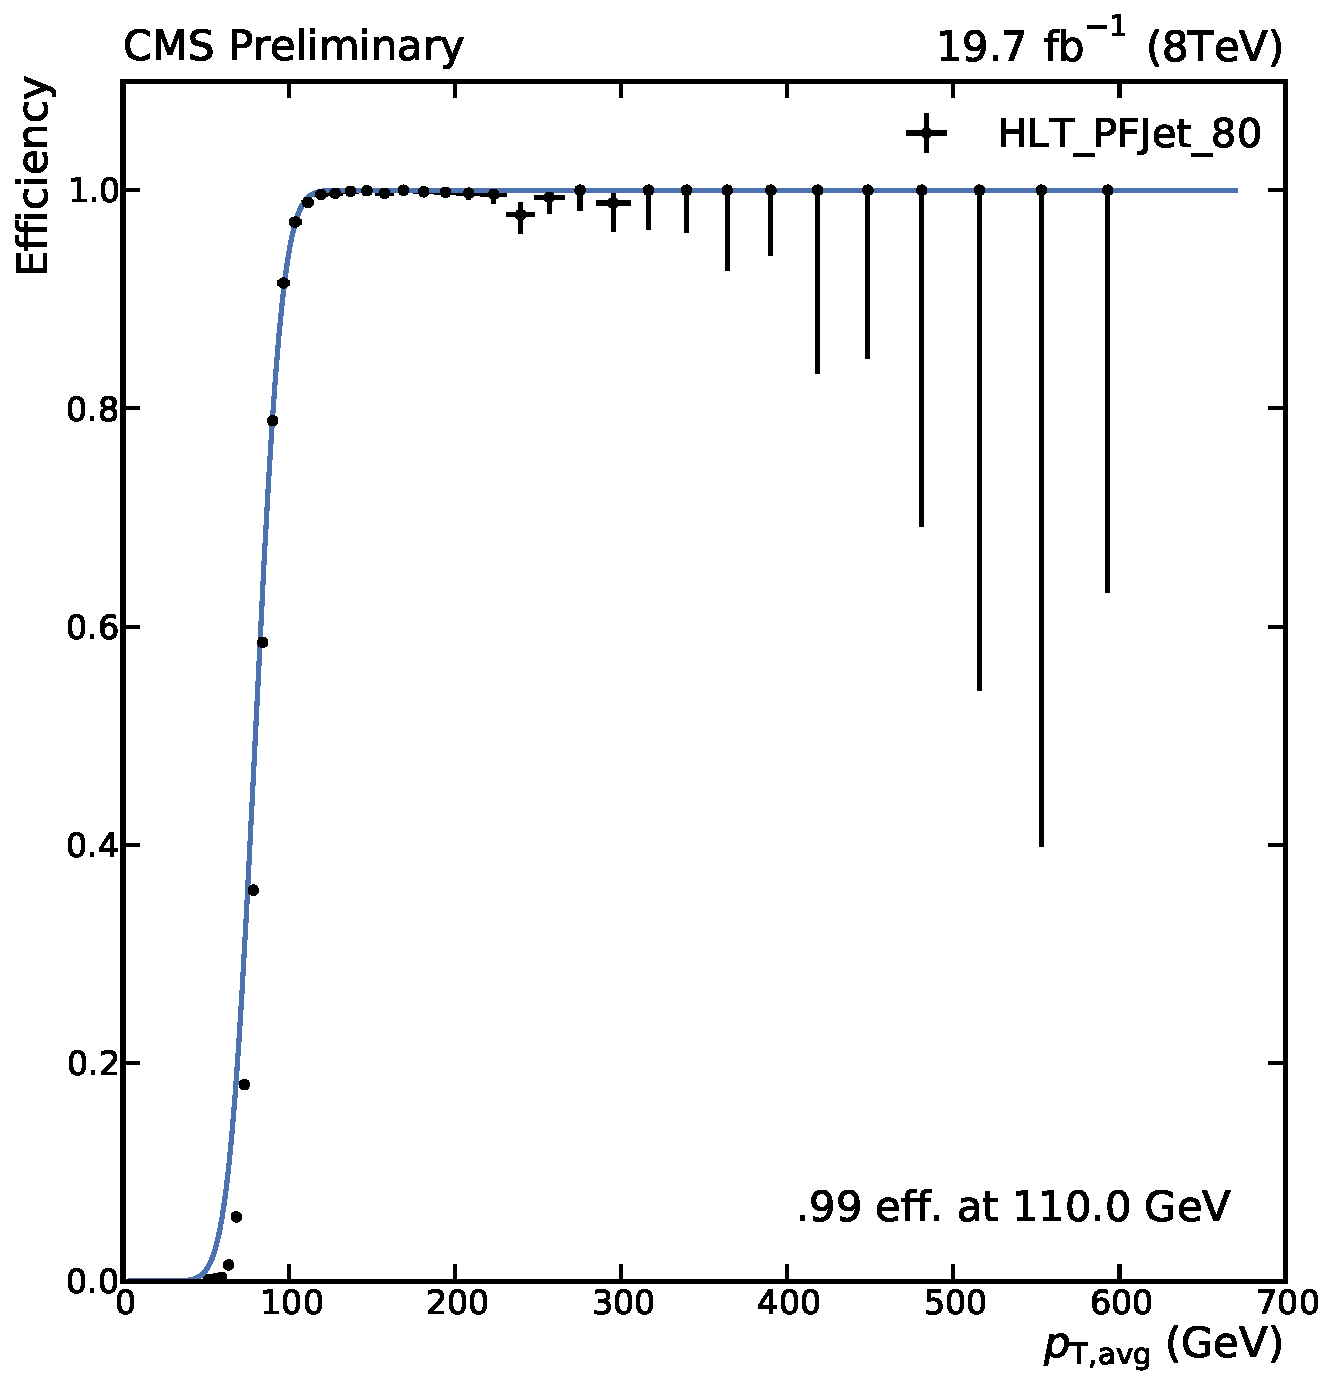
\includegraphics[width=0.45\textwidth]{figures/measurement/trigger_eff_hltpfjet80.pdf}\hfill
    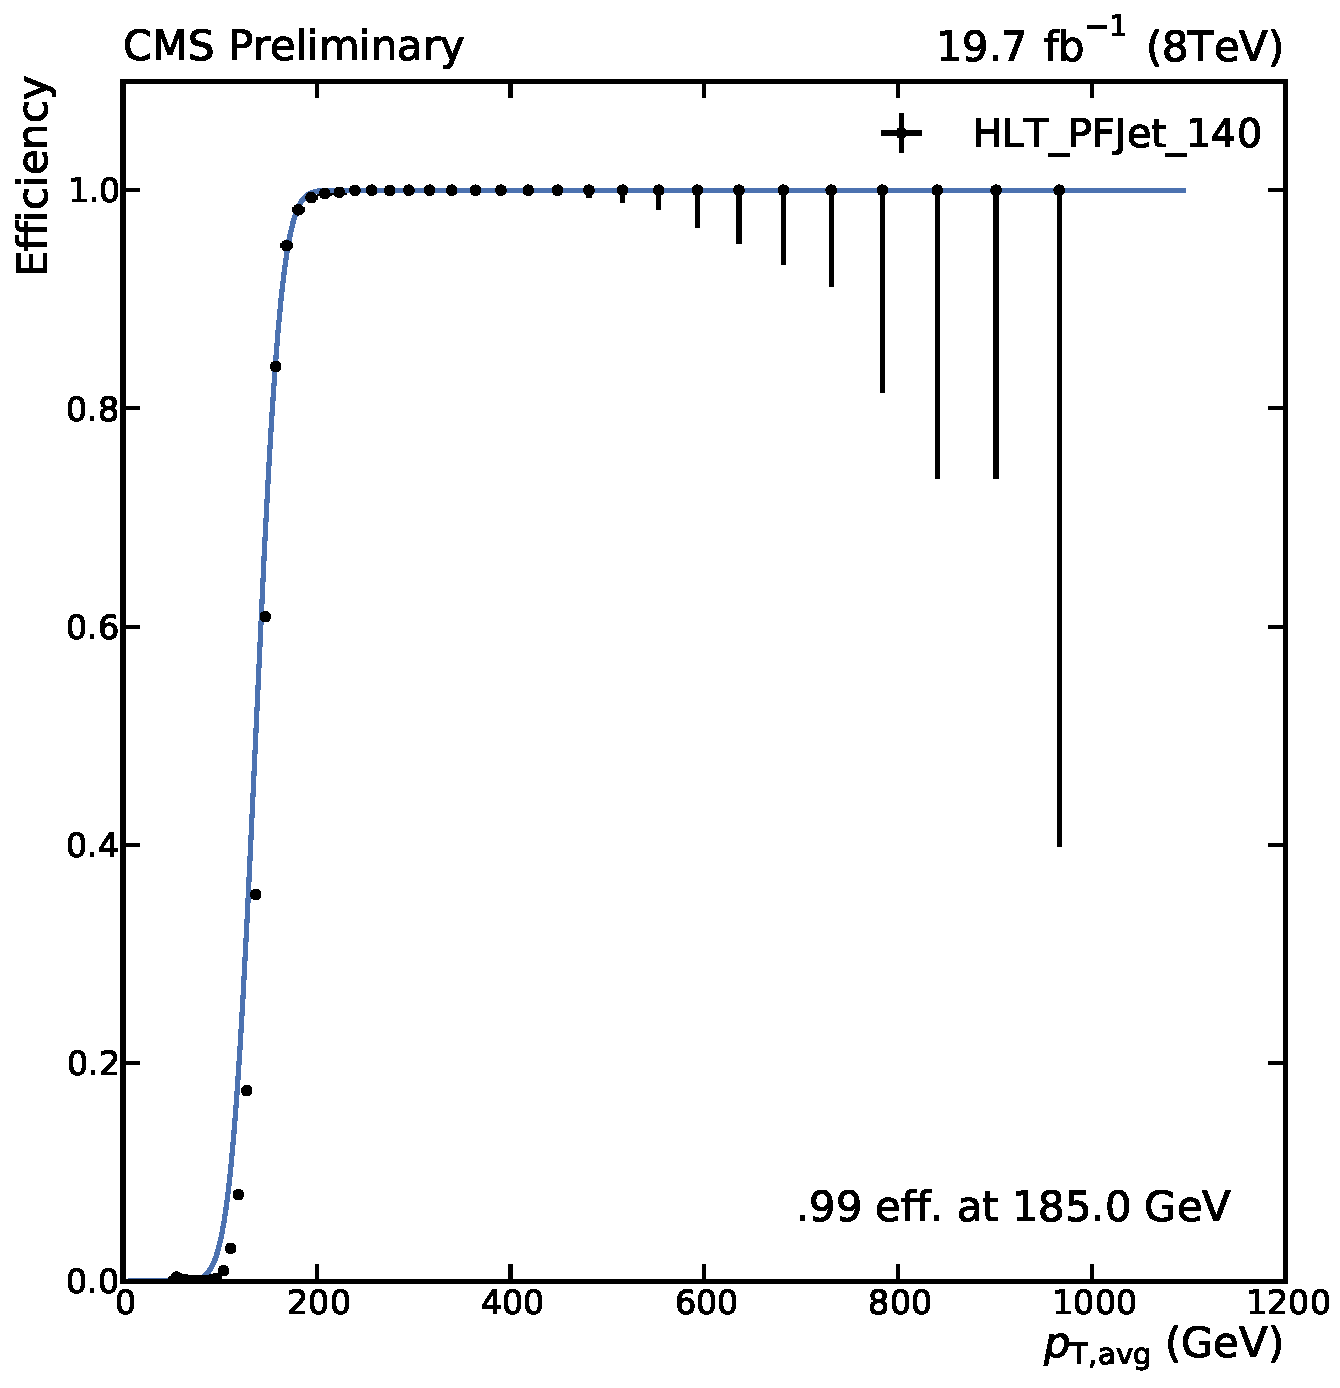
\includegraphics[width=0.45\textwidth]{figures/measurement/trigger_eff_hltpfjet140.pdf}
    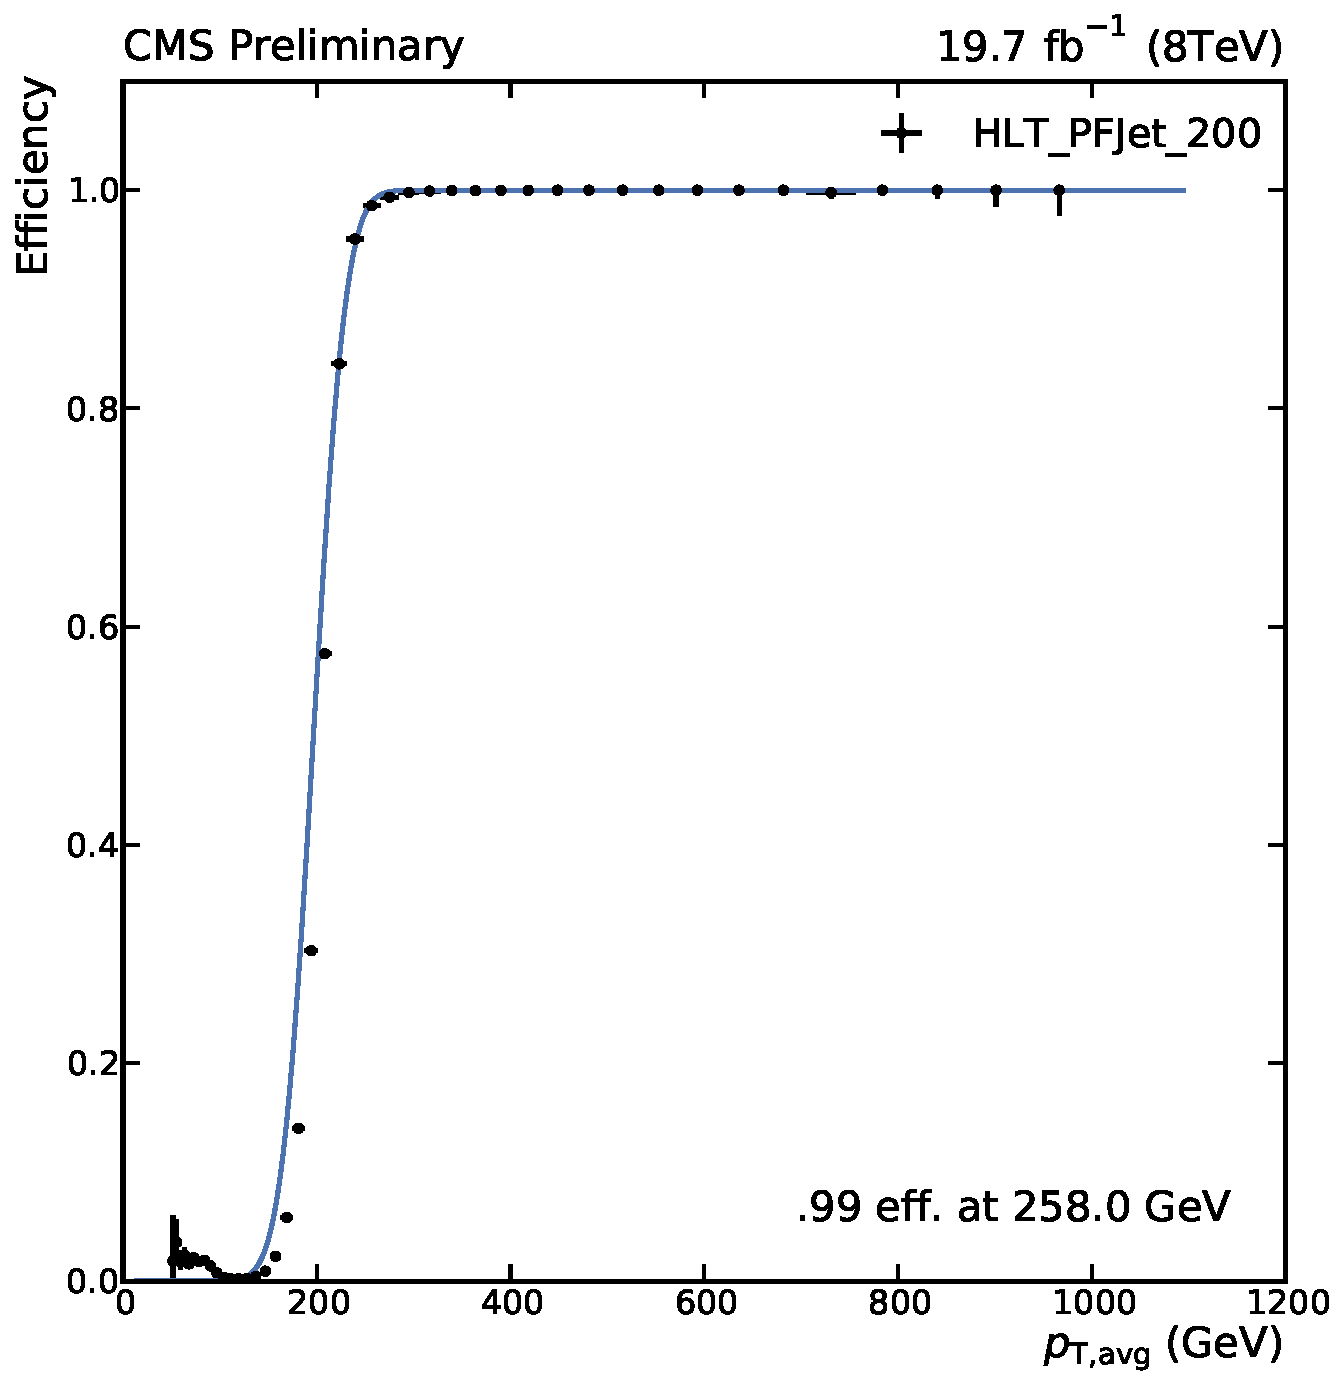
\includegraphics[width=0.45\textwidth]{figures/measurement/trigger_eff_hltpfjet200.pdf}\hfill
    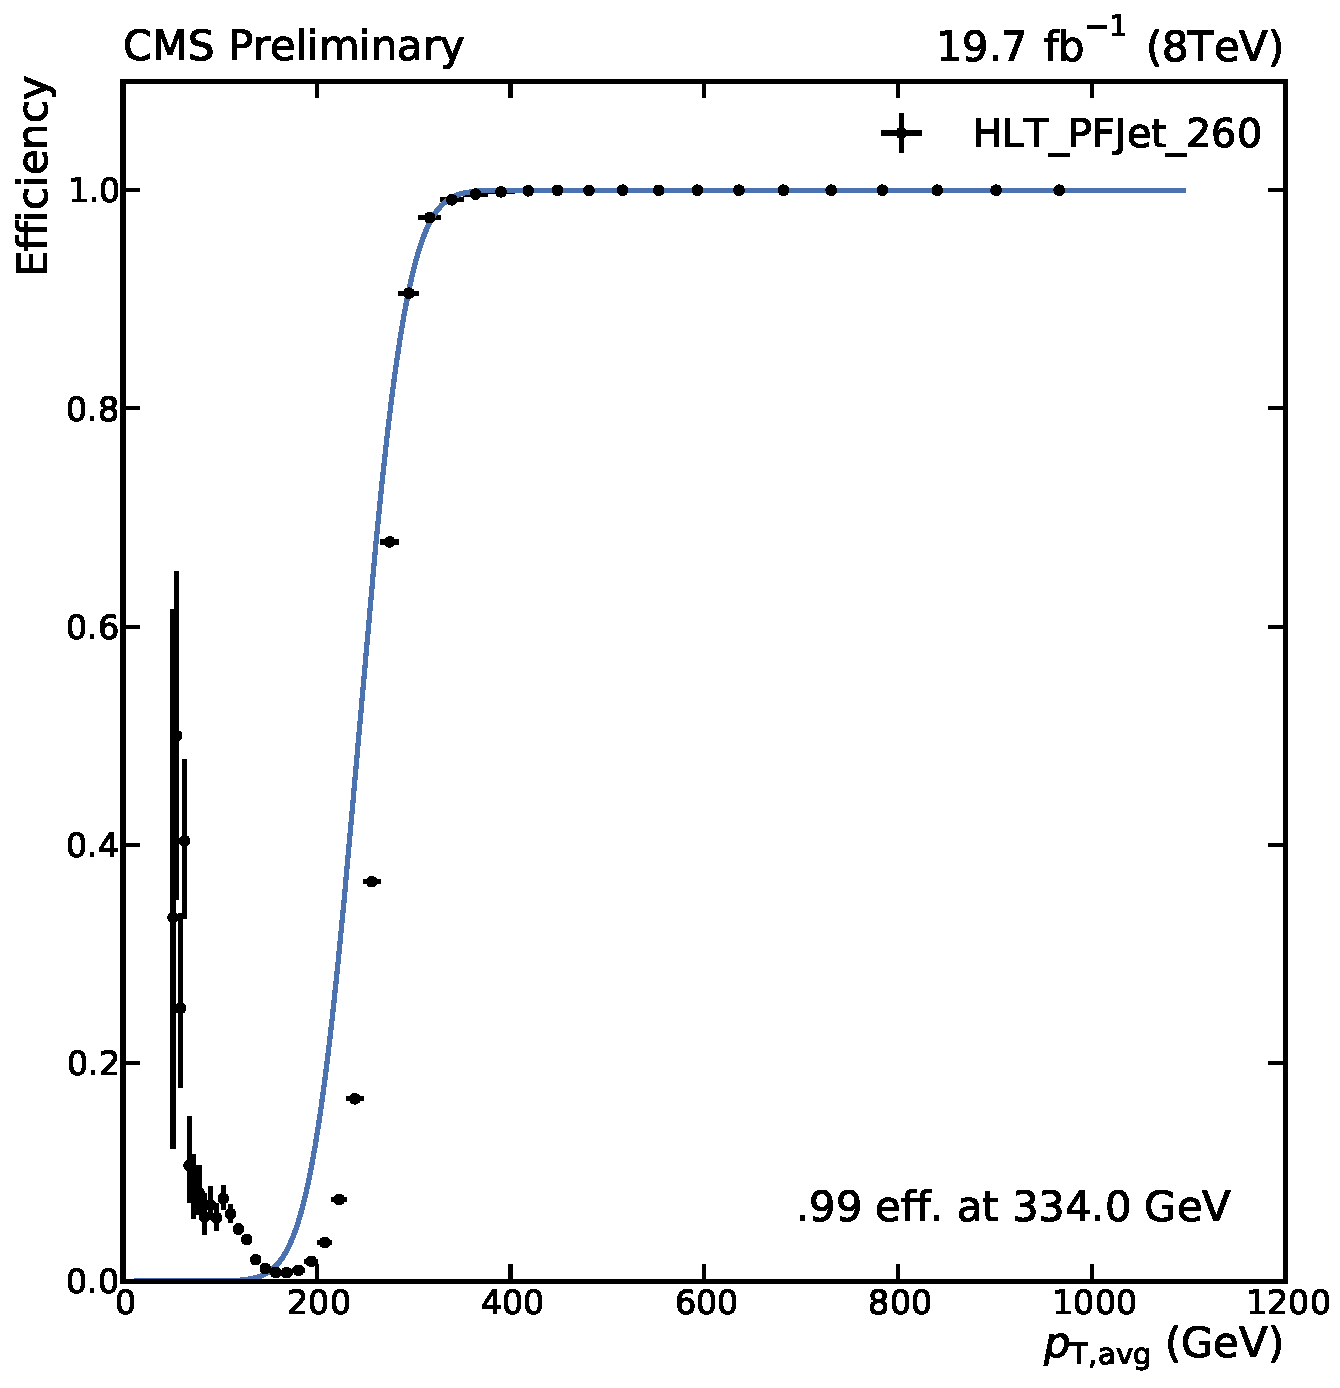
\includegraphics[width=0.45\textwidth]{figures/measurement/trigger_eff_hltpfjet260.pdf}
    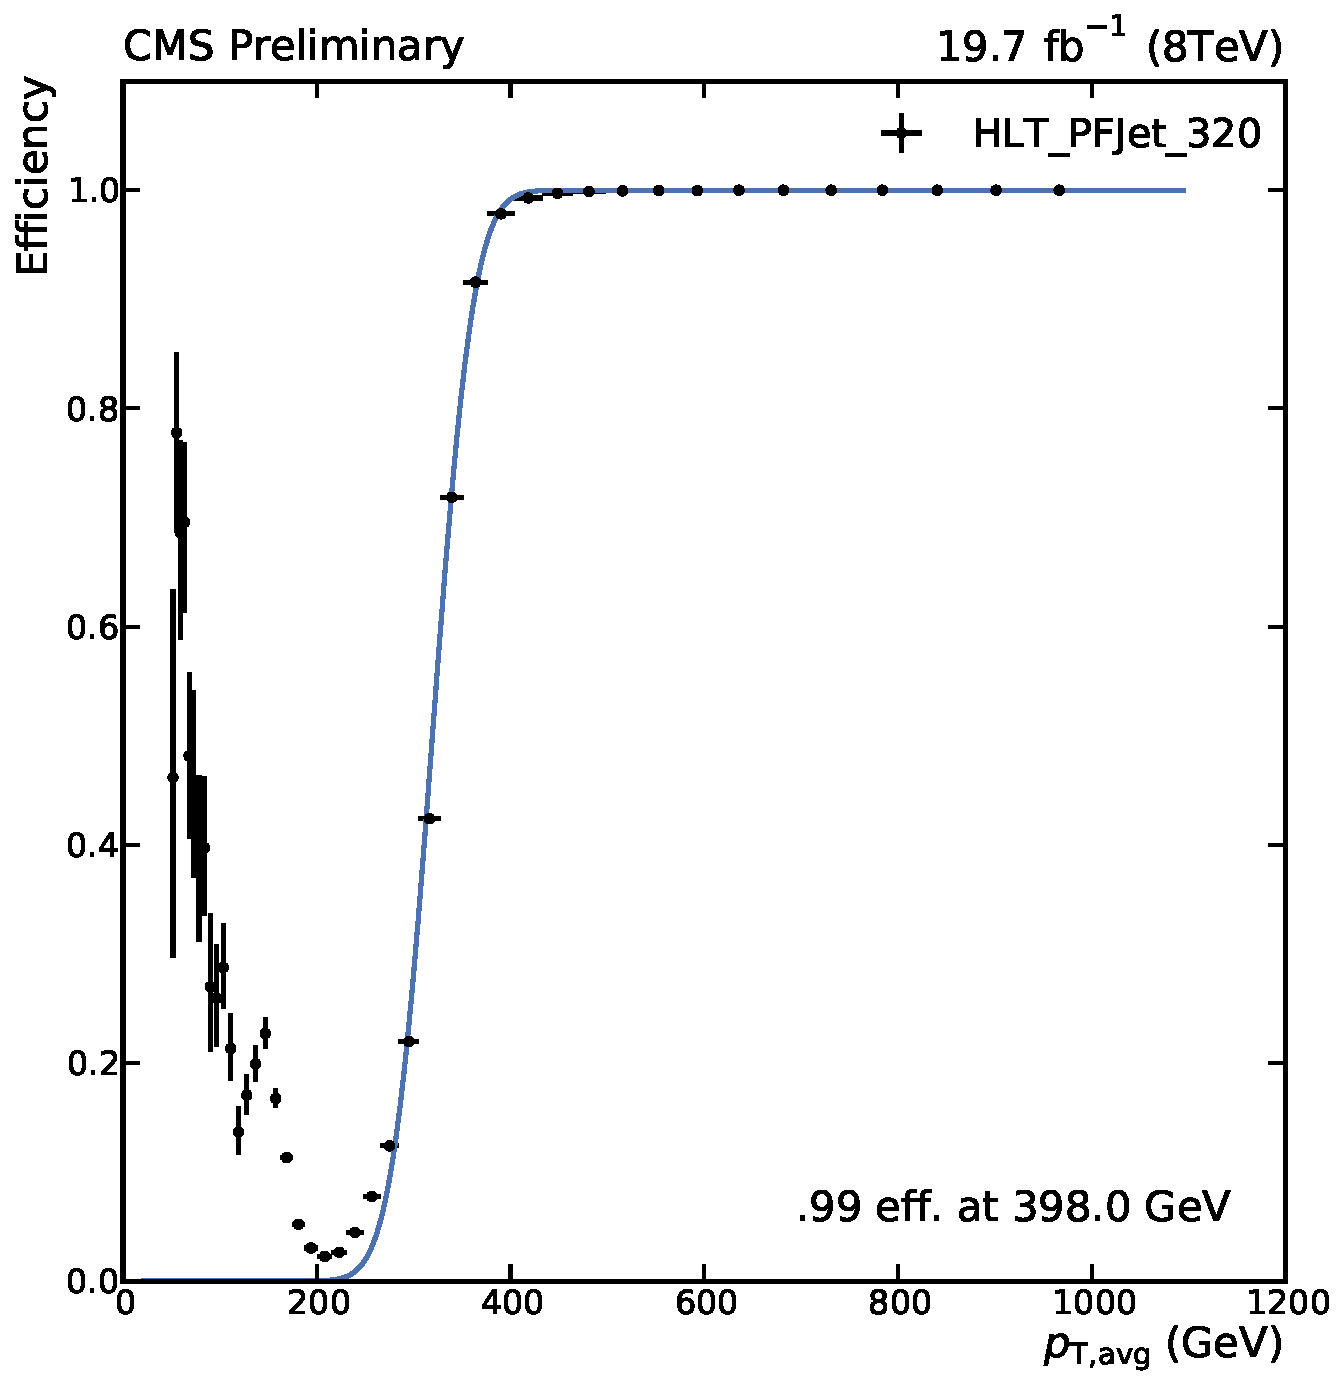
\includegraphics[width=0.45\textwidth]{figures/measurement/trigger_eff_hltpfjet320.pdf}\hfill
    \caption{Trigger efficiencies.}
    \label{fig:trigger_eff}
\end{figure}


Since the analysis is measuring the spectrum of the average \pt of the two
leading jets, it is neccessary to study the efficiency of the single jet trigger paths
versus \ptavg. Since all but the highest \pt trigger are prescaled, one cannot
simple divide the number of accepted events of one path through the number of
accecpted events of another path. The easiest approach is the scaling by the
effective luminosity seen by each trigger to normalize both triggers to the same
yield. For jet triggers this approach is undesired since the number of accepted
events per trigger fluctuates strongly with the prescales and may introduce
unncessary large statistical fluctuations. Therefore the trigger decision  of a
given path is always emulated starting from the next-lower trigger path by checking
if the L1 and HLT objects, which passed the lower trigger, would also
have fired for the next trigger path. This is possible since the objects, on which
the L1 and HLT decision is based, are stored as well. A set of events $S_1 = \left\{E_i | T_A (E_i) = true \right\}$
which was accepted  by the lower trigger path $T_A$ is used to determine the subset
$S_2 = \left\{E_i|T_A(E_i) \wedge  T_B(E_i) \right\}$ which would also pass the higher trigger 
$T_B$. The ratio of both event sets can be used to determine the efficiency as shown for each trigger
path in Figure~\ref{fig:trigger_eff} using the Equation~\ref{eq:trigger_eff}. 

\begin{equation}
\label{eq:trigger_eff}
    f_{\text{eff}} (x) = \frac{N(\left\{E_i|T_A(E_i) \wedge T_B(E_i), x)\right\}}{N(\left\{ E_i | T_A(E_i) = \text{true} \right\} , x)}
\end{equation}

The efficiency versus \ptavg is fitted using the sigmoid function~\ref{eq:trigger_eff_fit} describing
the turn-on behaviour of the trigger paths. Each trigger was used in a region in which the efficiency
is larger than $99\%$. The actual used trigger efficiency deviate slightly from the once shown in Table~\ref{tab:triggers}
since the used trigger eff. thresholds were measured for each \ystar and \yboost bin and the most
conservative value was used.


\begin{equation}
\label{eq:trigger_eff_fit}
    f_{\text{fit}} (x) = \frac{1}{2} \left( 1 + \erf \left(\frac{x-\mu}{\sqrt{2}\sigma}\right)\right)
\end{equation}



\subsection{Missing transverse energy cut}
\subsection{Jet ID selection}
\subsection{Detector acceptance cuts}

\section{Dijet Resolution}

\section{Unfolding}

\section{Uncertainties}
